\documentclass[xcolor=table]{beamer}

\usepackage[english]{babel}
\usepackage[utf8]{inputenc}
\usepackage{hyperref}
\usepackage{graphicx}
\usepackage{amssymb,amsmath}
\usepackage{array}
\newcolumntype{H}{>{\setbox0=\hbox\bgroup}c<{\egroup}@{}} %usado para esconder uma coluna na tabela
\usepackage[most]{tcolorbox}
\usepackage{ulem}
\usepackage{fancybox}%caixas de texto
\usepackage{xcolor}%caixas de texto
\usetheme{Ufscar}
\useinnertheme{rounded}
\setbeamertemplate{navigation symbols}{} %tira os símbolos de navegaçao dos slides
\setbeamertemplate{}[page number] %contador de slides
\setbeamersize{text margin left=0.30cm,text margin right=0.30cm}
\setbeamertemplate{frametitle continuation}{} %para de enumerar os slides que tem [allowframebreaks]

\usepackage{epsfig,psfrag}
\usepackage{epsfig,graphicx}

\usepackage{subcaption}

\usepackage{longtable}

\usepackage{tabularx} %usado para ajustar a largura da tabela na página
\usepackage{ltablex} % usa tabularx de forma similar ao longtable

\usepackage[Algoritmo]{algorithm}% http://ctan.org/pkg/algorithms
\usepackage{algpseudocode}% http://ctan.org/pkg/algorithmicx %use [noend] para não aparecer escrito "end funtion"

%#############################################################33
%Terceiro Caption para longtable
\usepackage{forloop,longtable}
\newcounter{count}
\setcounter{count}{1}
\makeatletter
\newbox\LT@secondhead
\def\endsecondhead{\LT@end@hd@ft\LT@secondhead}
\def\LT@output{%
	\ifnum\outputpenalty <-\@Mi
	\ifnum\outputpenalty > -\LT@end@pen
	\LT@err{floats and marginpars not allowed in a longtable}\@ehc
	\else
	\setbox\z@\vbox{\unvbox\@cclv}%
	\ifdim \ht\LT@lastfoot>\ht\LT@foot
	\dimen@\pagegoal
	\advance\dimen@-\ht\LT@lastfoot
	\ifdim\dimen@<\ht\z@
	\setbox\@cclv\vbox{\unvbox\z@\copy\LT@foot\vss}%
	\@makecol
	\@outputpage
	\ifvoid\LT@secondhead
	\setbox\z@\vbox{\box\LT@head}%
	\else
	\setbox\z@\vbox{\box\LT@secondhead}%
	\fi
	\fi
	\fi
	\global\@colroom\@colht
	\global\vsize\@colht
	\vbox
	{\unvbox\z@\box\ifvoid\LT@lastfoot\LT@foot\else\LT@lastfoot\fi}%
	\fi
	\else
	\setbox\@cclv\vbox{\unvbox\@cclv\copy\LT@foot\vss}%
	\@makecol
	\@outputpage
	\global\vsize\@colroom
	\ifvoid\LT@secondhead
	\copy\LT@head\nobreak
	\else
	\box\LT@secondhead\nobreak
	\fi
	\fi}
\makeatother
%Fim: Terceiro Caption para longtable
%############################################################################################

\title[Exame de Qualificação]{Crop field detection using graph-based image segmentation and contrastive learning}
\author[PPGCCS -- UFSCar]{Marciele de Menezes Bittencourt,Co-Orientador: Dr. Renato Moraes Silva, Orientador: Prof. Dr. Tiago A. Almeida}
 
\vfill
\date{\footnotesize}

%Rodapé com número de slide
\expandafter\def\expandafter\insertshorttitle\expandafter{%
  \hspace*{\fill}%
  \insertframenumber\,/\,\inserttotalframenumber}
 
%===== cor do rodapé=========
\definecolor{azulEscuro}{RGB}{50,50,255}
\setbeamercolor*{palette quaternary}{fg=white,bg=azulEscuro!30!black} %cor do rodapé %muda outras cores do template
%============================
 
\abovecaptionskip 0.01 \abovecaptionskip %espaço antes caption
\belowcaptionskip 0 \belowcaptionskip %espaço depois caption

\newcommand{\up}[1]{\raisebox{1.5ex}[0pt]{#1}}

\usepackage{multirow}%tabelas
\usepackage{rotating} %rotacionar texto na tabela

%%%%%%%%%%%%%%%%%%%%%%%%%%%%%%%%%%%%%%%%%%%%%%%%%%%%%%%%%%%%%%%%%
\setbeamertemplate{itemize subitem}{$\blacktriangleright$}
\setbeamertemplate{itemize subsubitem}{$\bullet$} %\diamond
%\setbeamertemplate{itemize item}[square] %altera o símbolo que inicia 
\setbeamertemplate{itemize subitem}[triangle] %altera o símbolo que inicia um subitem em uma lista
%\setbeamertemplate{itemize subsubitem}[circle] %altera o símbolo que inicia um subsubitem em uma lista
 %%%%%%%%%%%%%%%%%%%%%%%%%%%%%%%%%%%%%%%%%%%%%%%%%%%%%%%%%%%%%%%%%
 
 \graphicspath{%
 	{figs/}%
 }
\begin{document}

%=============================================
\begin{frame}
	\begin{center}

	\vspace{0.3in}

	\Large \textbf{Crop field detection using graph-based image segmentation and contrastive learning}

	\vspace{0.2in}

	{\large \textbf{Eduardo Garcia do Nascimento}}

	\vspace{0.2in}
	{\normalsize \textbf{Advisor: Prof. Dr. Tiago A. Almeida}}

	\vspace{0.2in}
	{\small{ Graduate Program in Computer Science\\  [-0.1in]Federal University of São Carlos -- UFSCar, Sorocaba}}

	{\small November / 2022}

	\end{center}
\end{frame}
%=============================================

%=============================================
\begin{frame}{\normalsize What is Precision Agriculture?}
    \centering
    \begin{tikzpicture}
        \node[anchor=south west] (image) at (0,0) {
            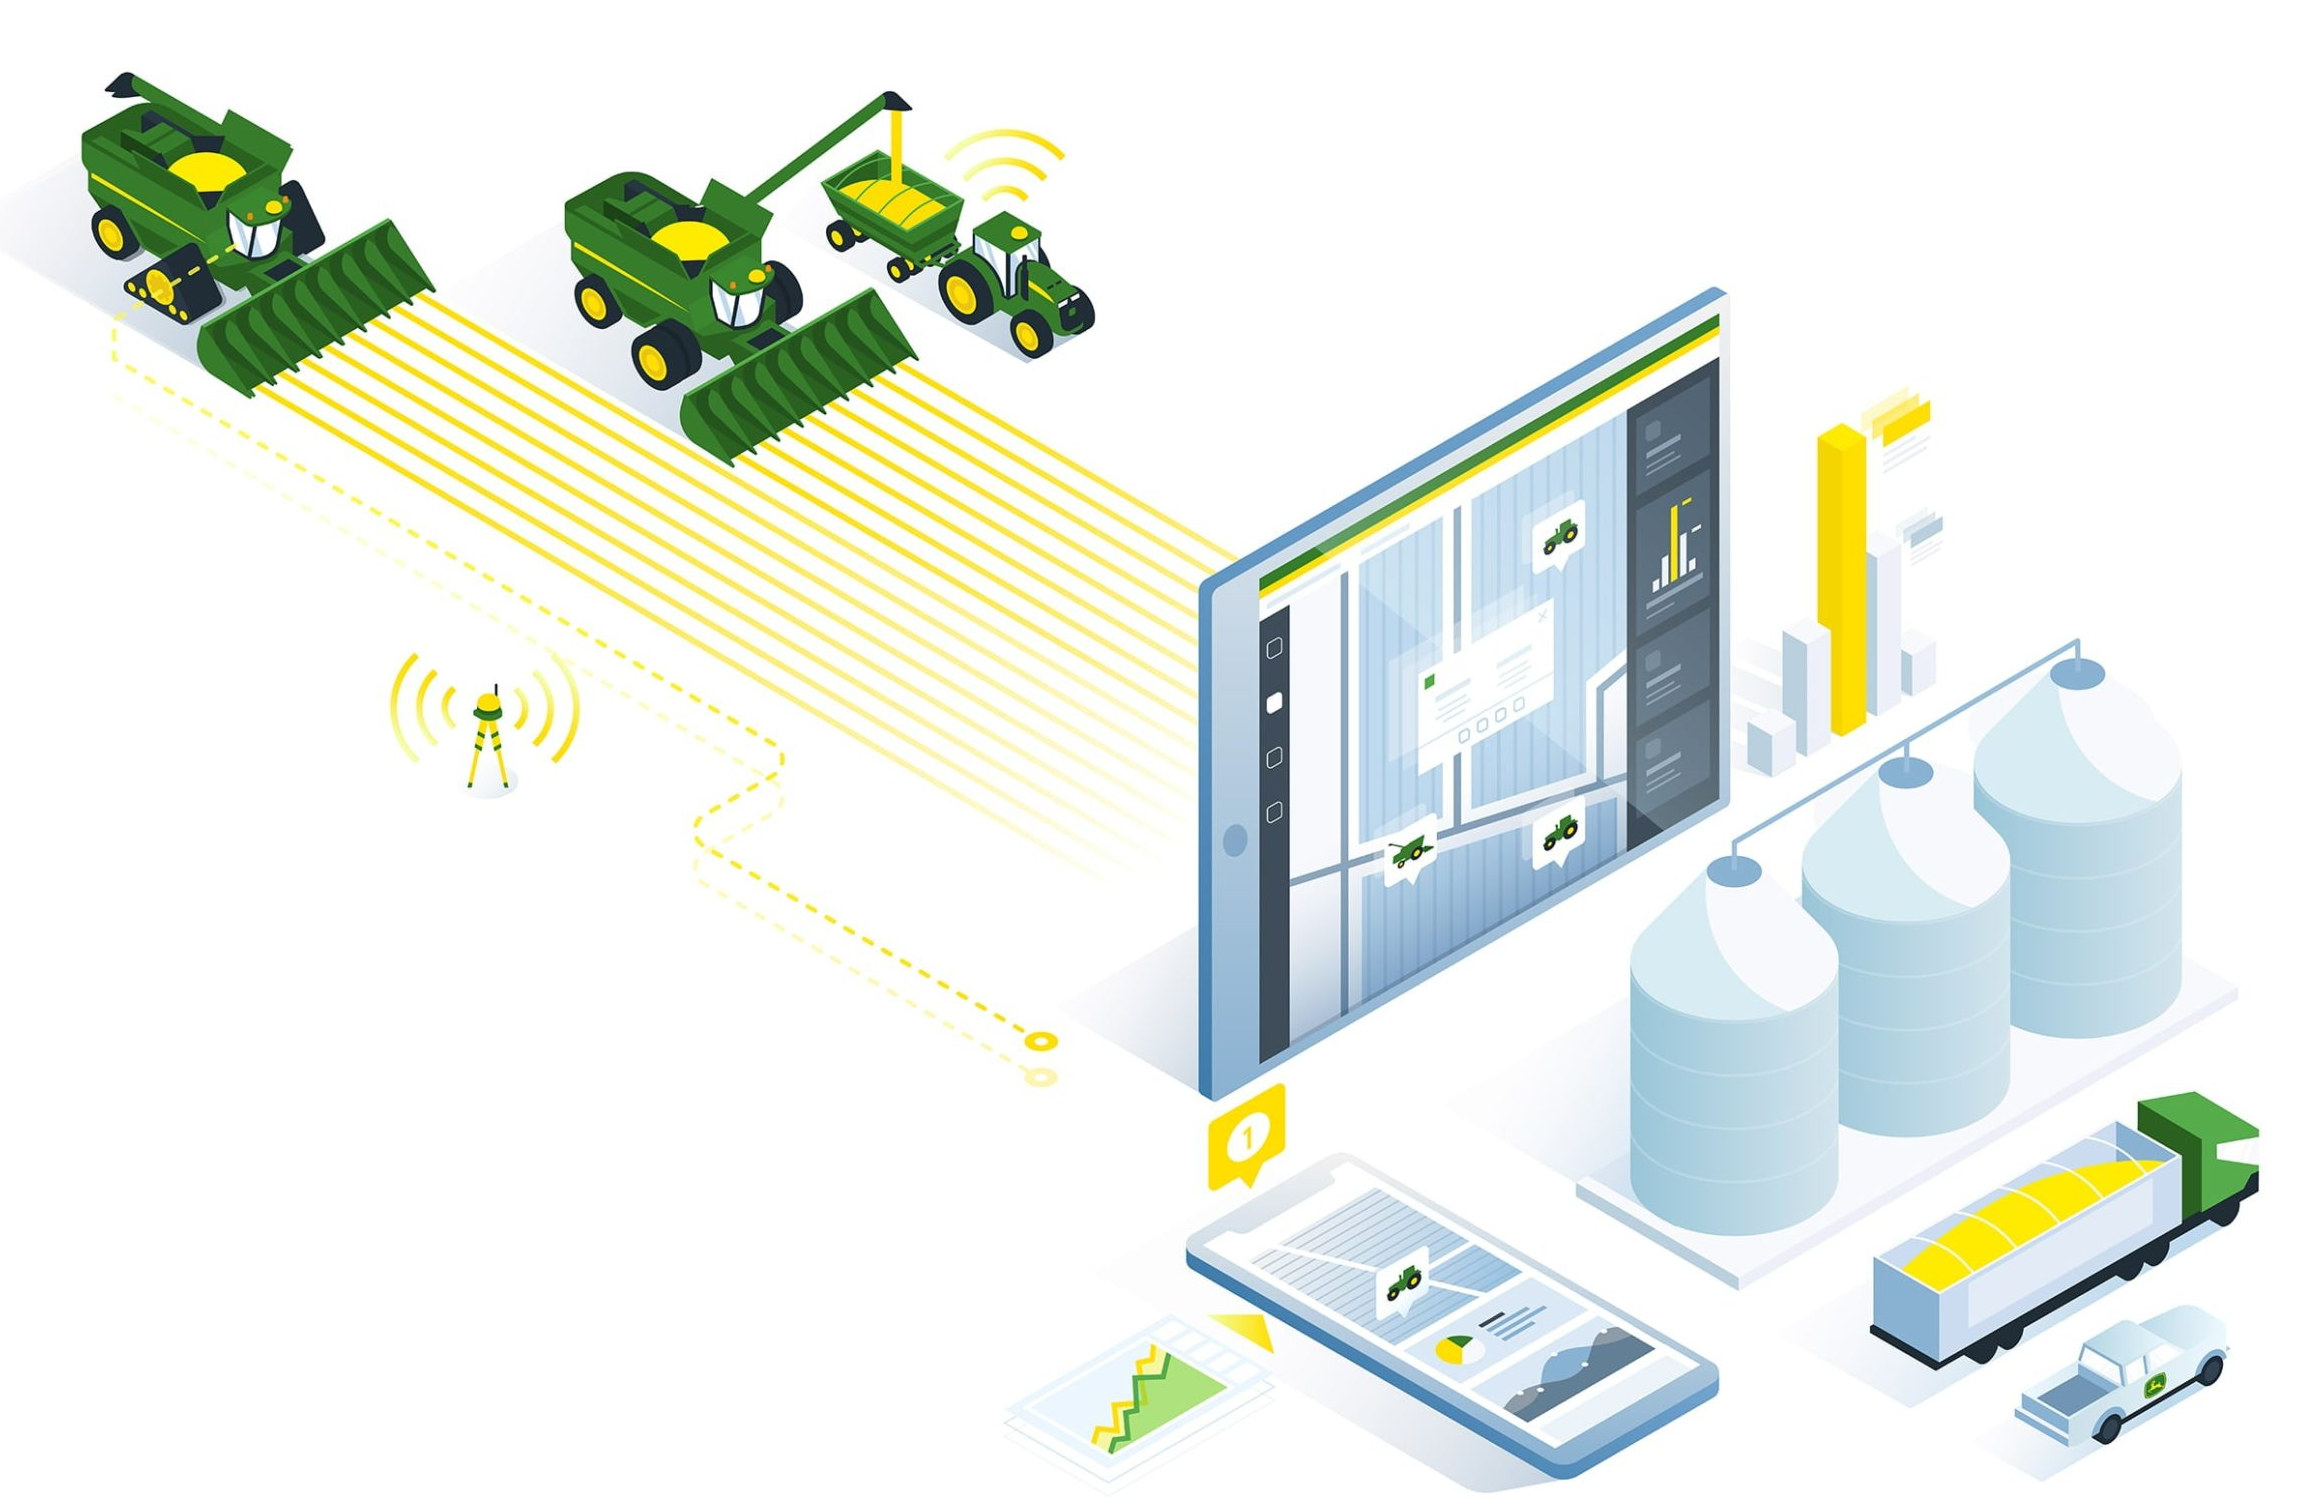
\includegraphics[height=6cm]{figs/precisionag.png}
        };
        \pause
        \node[align=center,red] at (image.center) {
            \begin{tcolorbox}[width=11cm,colback=yellow!5,colframe=yellow!75!black] A farming management concept based on observing, measuring and responding to variability in crops, adopting and optimizing technologies many times developed in other industries.\end{tcolorbox}
        };
    \end{tikzpicture}
	
    ~\flushright \tiny {Images extracted from John Deere website. Available at: \url{https://www.deere.com/}. Access on June 11, 2022}
	
\end{frame}
%=============================================

%=============================================
\begin{frame}{ \normalsize Remote Sensing in Precision Agriculture}
		
	\begin{columns}
		\column{0.6\textwidth}
		    \begin{tcolorbox}[colback=yellow!5,colframe=yellow!75!black]
		    A \textit{crop field} is the smallest observation unit designed by a farm based on the topography and mechanization plan. 
	        \end{tcolorbox}
	        
    		\begin{figure}[htb]
    			\centering
    			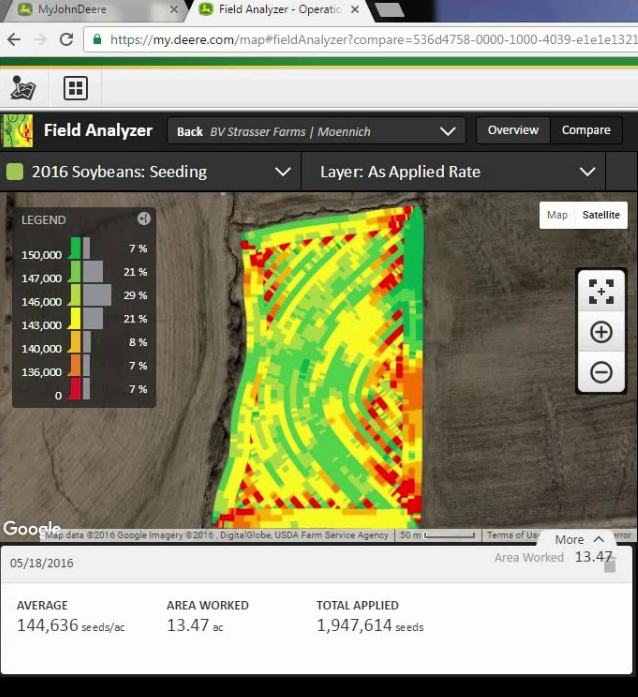
\includegraphics[height=3.5cm]{figs/fieldanalyzer.png}
    			\label{fig:textFieldAnalyzer}
    		\end{figure}

        \column{0.4\textwidth}

    		\begin{figure}[htb]
    			\centering
    			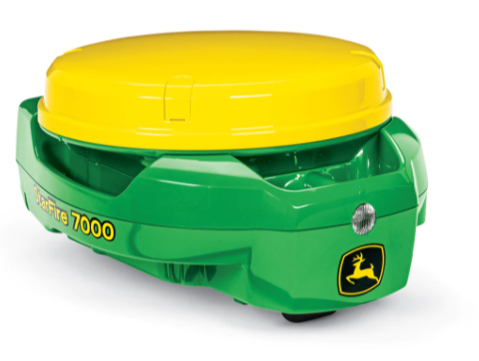
\includegraphics[height=3cm]{figs/gps.png}
    			\label{fig:gps}
    		\end{figure}
    		
    		\begin{figure}[htb]
    			\centering
    			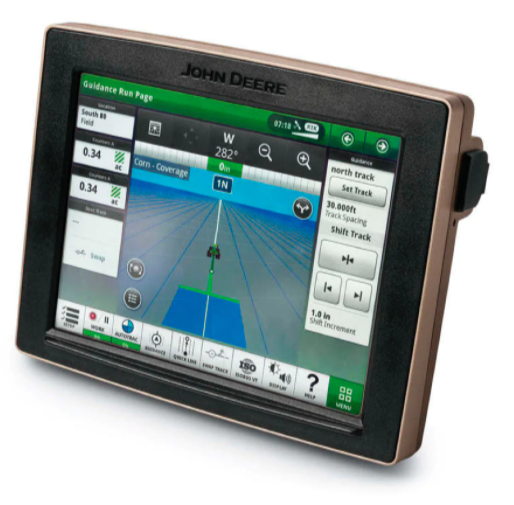
\includegraphics[height=3cm]{figs/display.png}
    			\label{fig:display}
    		\end{figure}

	\end{columns}
	~\flushright \tiny {Images extracted from John Deere website. Available at: \url{https://www.deere.com/}. Access on June 11, 2022})
	
\end{frame}
%=============================================

%=============================================
\begin{frame}{Boundary detection of crop fields}
	
	\begin{columns}
	\column{0.5\textwidth}

		\begin{figure}[htb]
			\centering
			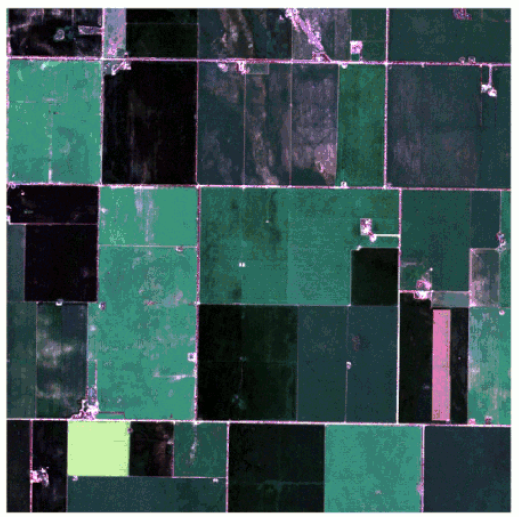
\includegraphics[height=4cm]{figs/field_nodetection.png}
			\label{fig:fieldNoDetection}
		\end{figure}
		\pause

	\column{0.5\textwidth}
		\begin{columns}
		\column{0.2\textwidth}
		
		\huge {$\Rightarrow$ }
		
		\column{0.8\textwidth}	
			\begin{figure}[htb]
				\centering
				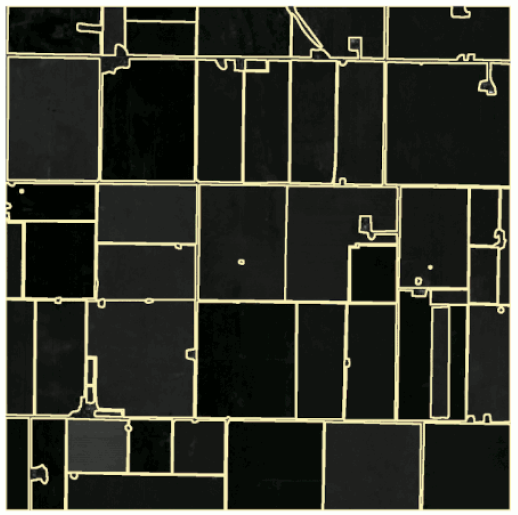
\includegraphics[height=4cm]{figs/field_detected.png}
				\label{fig:fieldDetected}
			\end{figure}
		\end{columns}
	\end{columns}
	
	~\flushright \tiny \cite{waldner2021}
	
\end{frame}
%=============================================

%=============================================
\begin{frame}{Related work}

\centering
	
\tikzstyle{block} = [draw, rectangle, 
    minimum height=2em, minimum width=6em, fill=orange, fill opacity=0.2, text opacity=1]

% The block diagram code is probably more verbose than necessary
\begin{tikzpicture}[auto, node distance=2.05cm]
    % We start by placing the blocks
    
    \node [block] (region) {Region-based}; % Low accuracy
    \pause
    \node [block, below right of=region] (edge) {Edge-based}; % Issues close to urban areas
    \draw [->](region) -- (edge);  
    \pause
    \node [block, below right of=edge] (hybrid) {Hybrid (Region + Edge)}; % best results compared to previous approaches but still very sensitive to seasonal changes
    \draw [->](edge) -- (hybrid);
    \pause
    \node [block, below right of=hybrid] (ml) {Machine Learning}; % really good performance 92% accuracy but high variability depending on the area it was applied
    \draw [->](hybrid) -- (ml);
    \pause
    \node [block, below right of=ml] (dl) {Deep Learning}; % CNNs, including U-Net with semantic segmentation and customized improvements however not enough labeled samples 
    \draw [->](ml) -- (dl);
 \end{tikzpicture}
	
		
\end{frame}
%=============================================

%=============================================
\begin{frame}{Problem}
	
	\begin{tcolorbox}[colback=red!5,colframe=red!75!black]
		Manually drawing field boundaries is a time-consuming and error-prone task.
	\end{tcolorbox}
	
	\begin{tcolorbox}[colback=red!5,colframe=red!75!black]
		The state-of-the-art automatic methods use deep learning to detect field boundaries but they need a significant number of labeled samples to work appropriately.
	\end{tcolorbox}
	
	\begin{tcolorbox}[colback=red!5,colframe=red!75!black]
		This requirement makes the application of deep learning restricted to limited areas of the globe. 
	\end{tcolorbox}
		
\end{frame}
%=============================================

%=============================================
\begin{frame}{Contrastive Learning}
	
	\begin{columns}
		\column{0.6\textwidth}

		\begin{figure}[htb]
      			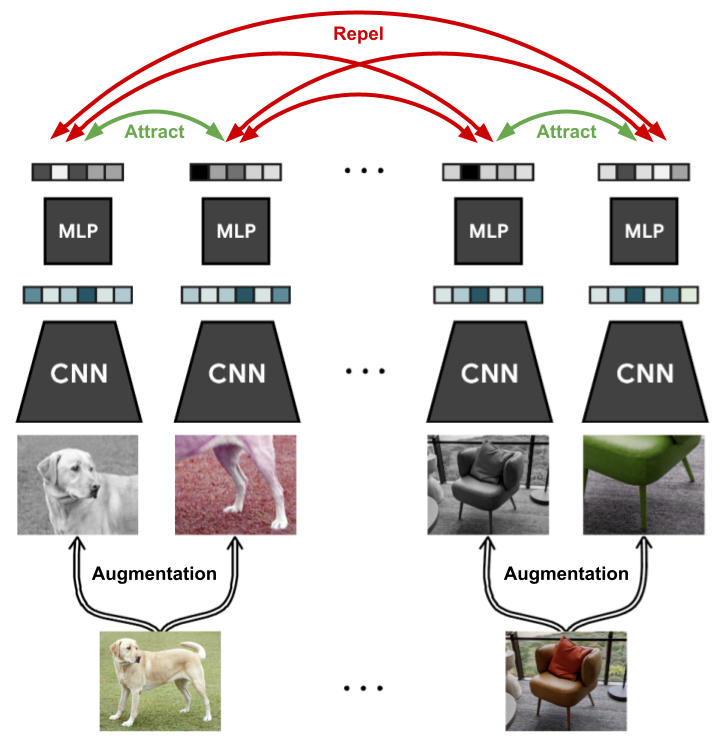
\includegraphics[height=5cm]{figs/contrastive_learning.png}
      			\label{fig:simCLR}
		\end{figure}
		~\flushright \tiny \cite{chen2020}
	
		\column{0.4\textwidth}
  
		\pause
 
		Steps: \\
		\begin{itemize}
			\item Data augmentation
			\item Encoding
			\item Loss minimization
		\end{itemize}
	    
		\bigskip
	
	\end{columns}

\end{frame}
%=============================================

%=============================================
\begin{frame}{Contrastive Loss}
	
	\centering
	
	\begin{equation}
	\ell_{(i,j)}=-\log{\frac{\exp{\left(sim(\boldsymbol{z}_i,\boldsymbol{z}_j)/\tau\right)}}{\sum_{k=1}^{2N}\mathbf{}_{[k\neq i]}\exp{\left(sim(\boldsymbol{z}_i,\boldsymbol{z}_k)/\tau\right)}}}
	\end{equation}
	~\flushright \tiny \cite{chen2020})
\end{frame}
%=============================================

%=============================================
\begin{frame}{Contrastive Learning - Main methods}
    
    \begin{columns}
        \column{0.5\linewidth}
            \begin{itemize}
        		\item SimCLR~\cite{chen2020}
        		\begin{itemize}
        		    \item Developed by Google Research
        		    \item Strong data augmentation
        		    \item Larger batch size
        		    \item MLP projection head
        		\end{itemize}
        	\end{itemize}
    	\column{0.5\linewidth}
    	    \begin{itemize}
        		\item MoCo~\cite{he2020}
        		\begin{itemize}
        		    \item Developed by Facebook AI Research
        		    \item Moving average encoder
        		    \item Dynamic dictionary
        		\end{itemize}
    	    \end{itemize}
	\end{columns}
\end{frame}
%=============================================

%=============================================
\begin{frame}{Hypotheses}

	\begin{tcolorbox}[colback=blue!5,colframe=blue!75!black]
		As contrastive learning based methods require much fewer labeled samples than state-of-the-art deep learning models, their employment to detect field boundaries can lead to competitive results with minimal accuracy loss, demanding just a few labeled samples.
	\end{tcolorbox}
		
\end{frame}
%=============================================

%=============================================
\begin{frame}\frametitle{Implementation Proposal} 
	
	\begin{itemize}
		
		\item Labeling
		\begin{itemize}
			\item Labeled data from boundaries manually drawn by John Deere customers.
			\item Alternatively, operation data can be used to estimate boundaries.
		\end{itemize}
        
        \item Remote sensing
		\begin{itemize}
			\item Sentinel II satellite images.
			\item Other sources to be evaluated during the research.
		\end{itemize}
		
		\item Model
		\begin{itemize}
			\item Train model using few samples of high-quality labeled data.
			\item Graph-based segmentation~\cite{felzenszwalb2004}.
		\end{itemize}
	\end{itemize}
	
\end{frame}
%=============================================

%=============================================
\begin{frame}{Implementation Proposal}
	
	\centering
	
\tikzstyle{block} = [draw, rectangle, 
    minimum height=3em, minimum width=6em, fill=orange, fill opacity=0.2, text opacity=1]

% The block diagram code is probably more verbose than necessary
\begin{tikzpicture}[auto, node distance=4cm]
    % We start by placing the blocks
    
    \node [block] (data) {1. Data Processing};
    \node [block, right of=data] (training) {2. Model Training};
    \node [block, right of=training] (segmentation) {3. Segmentation};
    % We draw an edge between the controller and system block to 
    % calculate the coordinate u. We need it to place the measurement block. 
    \draw [->](data) -- (training);
    \draw [->](training) -- (segmentation);
\end{tikzpicture}
\end{frame}
%=============================================

%=============================================
\begin{frame}\frametitle{Implementation Proposal - Data Processing} 

	\begin{figure}[htb]
		\centering
		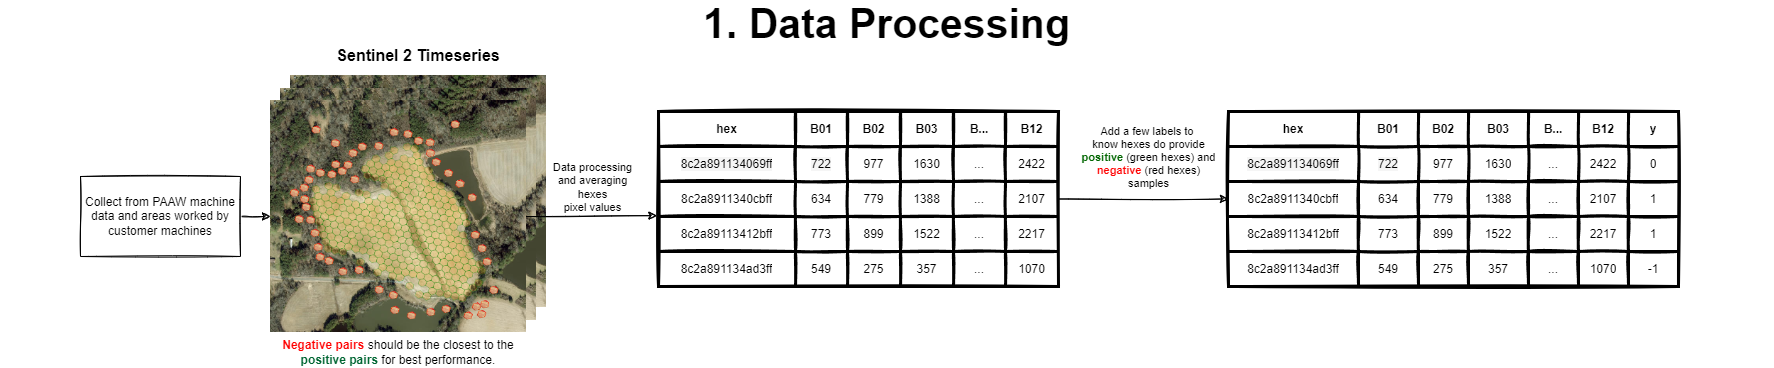
\includegraphics[width=12cm]{Exame de Qualificação/figs/1.png}
		\label{fig:data}
	\end{figure}
	~\flushright \tiny~ {Source: the author}
\end{frame}
%=============================================

%=============================================
\begin{frame}\frametitle{Implementation Proposal - Model Training} 

	\begin{figure}[htb]
		\centering
		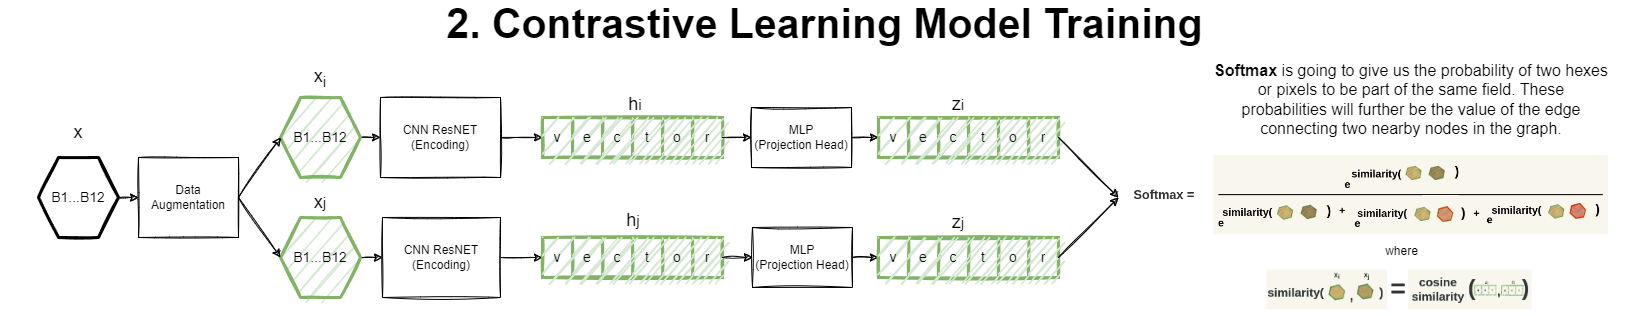
\includegraphics[width=12cm]{Exame de Qualificação/figs/2.png}
		\label{fig:model}
	\end{figure}
	~\flushright \tiny~ {Source: the author}
\end{frame}
%=============================================

%=============================================
\begin{frame}\frametitle{Implementation Proposal - Segmentation} 

	\begin{figure}[htb]
		\centering
		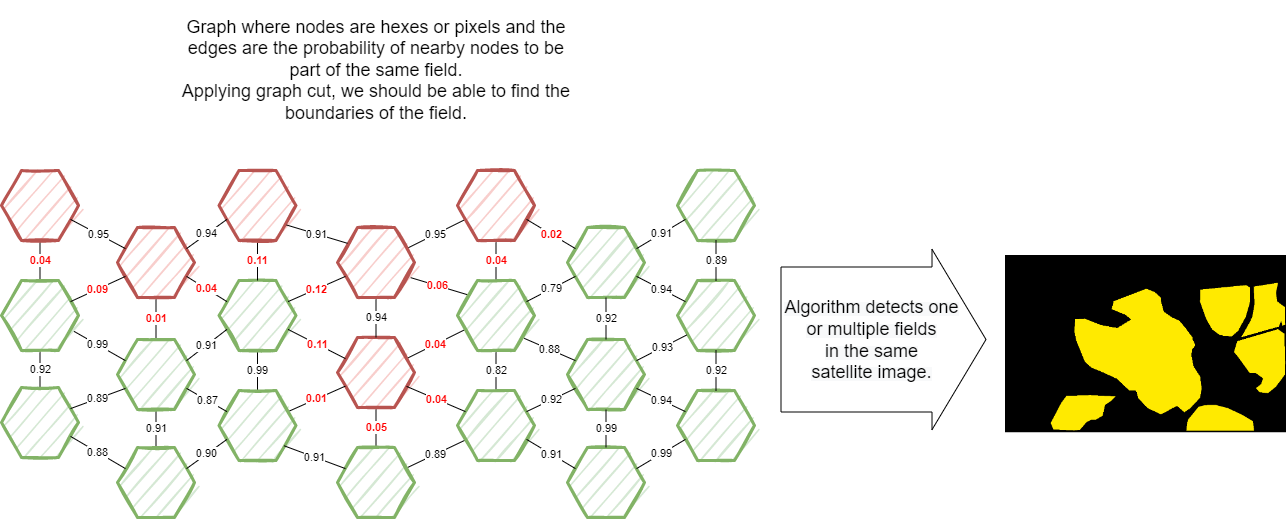
\includegraphics[width=12cm]{Exame de Qualificação/figs/3.png}
		\label{fig:segmentation}
	\end{figure}
	~\flushright \tiny~ {Source: the author}
\end{frame}
%=============================================

%=============================================
\begin{frame}{Materials and methods - SimCLR}
    
    \begin{columns}
        \column{0.5\linewidth}
        \centering
            \begin{tcolorbox}[width=6cm,colback=yellow!5,colframe=yellow!75!black]
            SimCLR will be employed since it outperforms other contrastive learning methods in accuracy as well as it makes an efficient use of memory and CPU resources.
            \end{tcolorbox}
        \column{.5\linewidth}
            \centering
            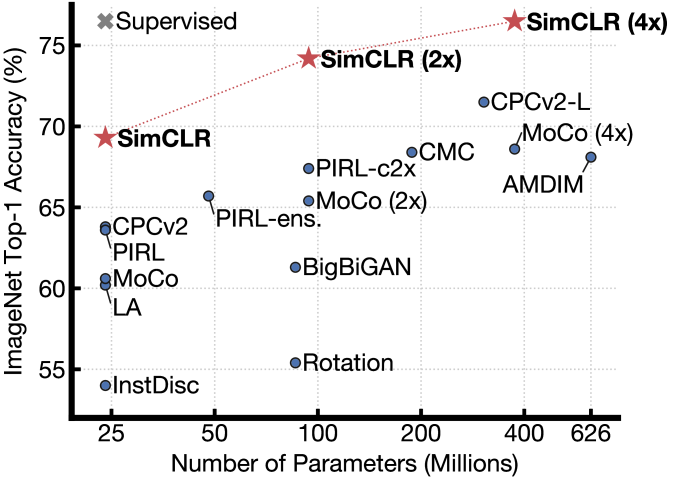
\includegraphics[width=5cm]{figs/simclr_chart_original.png}
            \tiny~\cite{chen2020}
    \end{columns}
\end{frame}
%=============================================

%=============================================
\begin{frame}{Materials and methods - H3}
    \begin{columns}[t]
        \column{.5\textwidth}
            \centering
            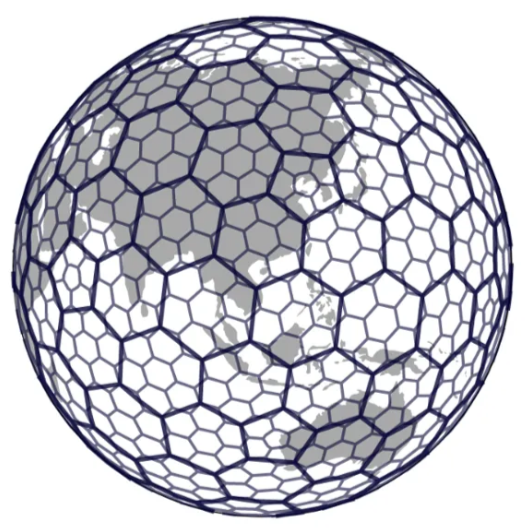
\includegraphics[width=3cm]{Exame de Qualificação/figs/h3-globe.png}
            \\\tiny~Division of the globe in hexagons
            \\~\\
            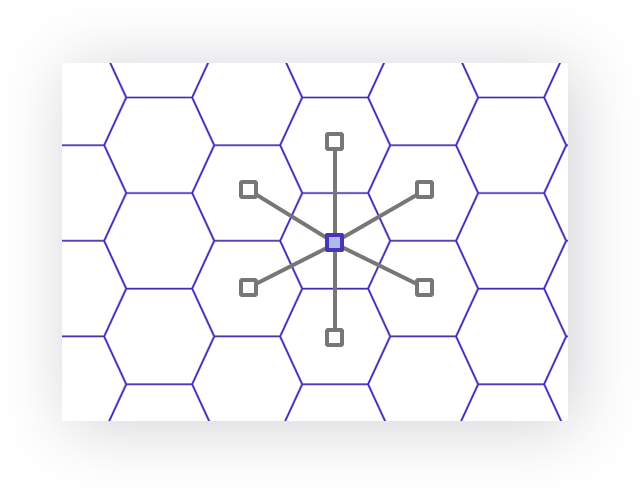
\includegraphics[width=3cm]{Exame de Qualificação/figs/h3-distances.png}
            \\\tiny~Distance from a hexagon to its neighbors
        \column{.5\textwidth}
            \centering
            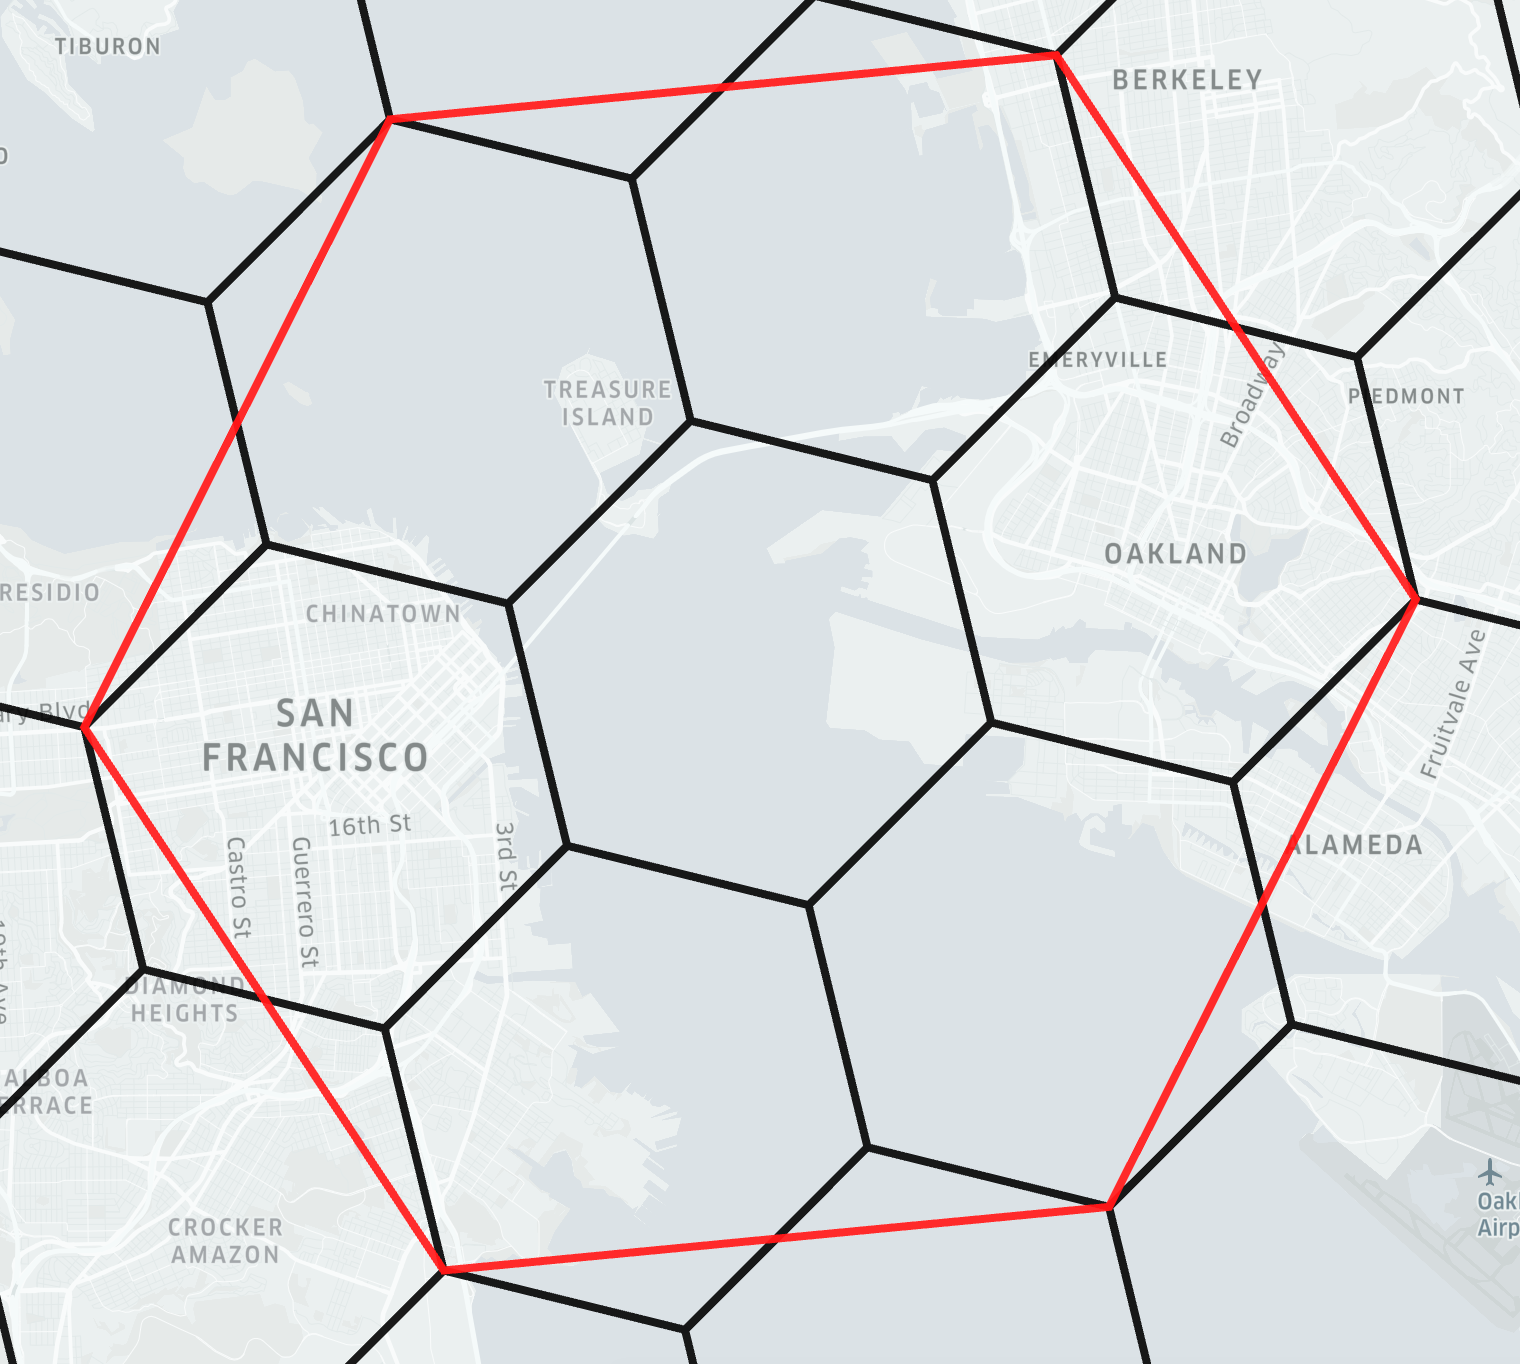
\includegraphics[width=3cm]{Exame de Qualificação/figs/h3-parent-child.png}
            \\\tiny~Hierarchical subdivision in smaller hexes
            \\~\\
            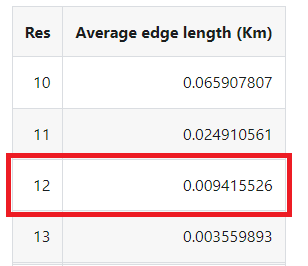
\includegraphics[width=3cm]{Exame de Qualificação/figs/h3-table.png}
            \\\tiny~Level 12 average edge length
    \end{columns}
    ~\flushright \tiny {Images extracted from H3 Geo website. Available at: \url{https://h3geo.org/}. Access on June 11, 2022}
\end{frame}
%=============================================

%=============================================
\begin{frame}{Materials and methods - In-Field H3 L12}
    \centering
    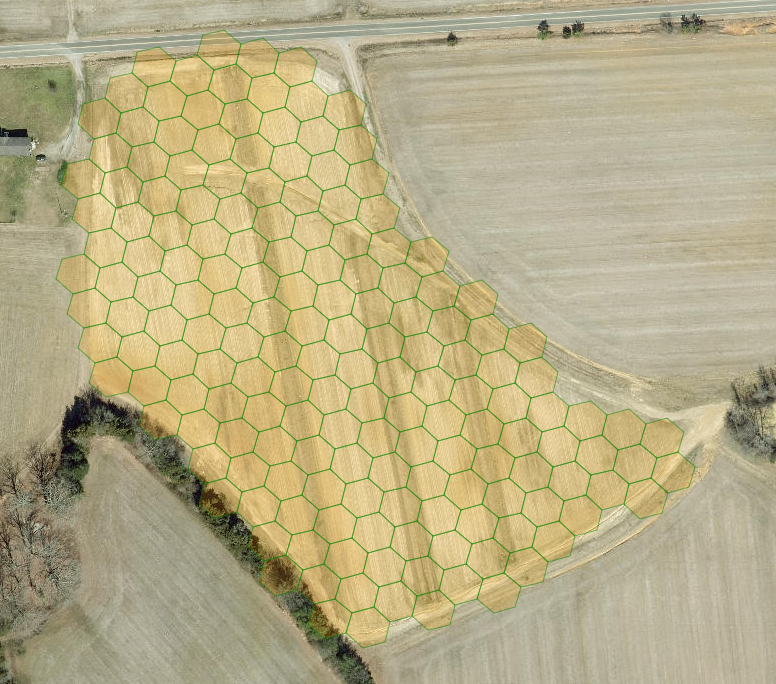
\includegraphics[width=6cm]{Exame de Qualificação/figs/h3-field.png}
    \\\tiny~Hexes covering an inferred crop field
    ~\flushright \tiny {Source: The author}
\end{frame}
%=============================================

%=============================================
\begin{frame}{Materials and methods - Validation}

	\begin{itemize}
		\item The validation will follow the metrics~\cite{sokolova2009} employed by related state-of-the-art work~\cite{waldner2021}.
	\end{itemize}		

	\begin{itemize}
	    \item Thematic accuracy
		\begin{itemize}
			\item Pixel or Region-based accuracies.
			\item Overall, user's and producer's accuracy.
			\item Matthew's correlation coefficient (MCC).
		\end{itemize}
		
		\item Geometric accuracy
		\begin{itemize}
			\item Boundary similarity.
			\item Location similarity.
			\item Over and Under segmentation rates.
		\end{itemize}
	\end{itemize}
		
\end{frame}
%=============================================

%=============================================

\begin{frame}[fragile]
\frametitle{Timeline}

\begin{center}
	\begin{tiny}
    \begin{longtable}{|c|c|c|c|c|c|c|c|c|c|c|c|c|c|}
    \hline
   & \multicolumn{4}{c|}{First year} & \multicolumn{4}{c|}{Second year} \\
    \cline{2-9}
    \up{Tasks} &1\textordmasculine T&2\textordmasculine T&3\textordmasculine T&4\textordmasculine T
	&1\textordmasculine T&2\textordmasculine T&3\textordmasculine T&4\textordmasculine T\\
    \hline
    \multicolumn{1}{|c|}{\begin{tabular}[c]{@{}c@{}c@{}}Bibliographical \\review\\{ } \end{tabular}}&\cellcolor[gray]{.1}&\cellcolor[gray]{.1}&\cellcolor[gray]{.1}&\cellcolor[gray]{.4}&\cellcolor[gray]{.8}&\cellcolor[gray]{.8}&\cellcolor[gray]{.8}&\cellcolor[gray]{.8}\\
    \hline
    \multicolumn{1}{|c|}{\begin{tabular}[c]{@{}c@{}c@{}}Extraction of remote sensing\\images and\\manually drawn boundaries \end{tabular}}&&\cellcolor[gray]{.1}&\cellcolor[gray]{.1}&\cellcolor[gray]{.4}&&&&\\   
    \hline
    \multicolumn{1}{|c|}{\begin{tabular}[c]{@{}c@{}c@{}}Study of SimCLR\\ and similar\\ contrastive learning techniques\end{tabular}}&&\cellcolor[gray]{.1}&\cellcolor[gray]{.1}&\cellcolor[gray]{.4}&&&&\\ 
    \hline
    \multicolumn{1}{|c|}{\begin{tabular}[c]{@{}c@{}c@{}}Modeling, build \\and planning of\\required adaptations\end{tabular}}&&&\cellcolor[gray]{.1}&\cellcolor[gray]{.4}&\cellcolor[gray]{.8}&&&\\
        \hline
    \multicolumn{1}{|c|}{\begin{tabular}[c]{@{}c@{}c@{}}Execution of the model\\and evaluation \\of first results\end{tabular}}&&&&&\cellcolor[gray]{.8}&\cellcolor[gray]{.8}&&\\
        \hline
    \multicolumn{1}{|c|}{\begin{tabular}[c]{@{}c@{}c@{}}Further experiments based on\\the evaluation of\\the first results\end{tabular}}&&&&&&\cellcolor[gray]{.8}&\cellcolor[gray]{.8}&\\
        \hline
    \multicolumn{1}{|c|}{\begin{tabular}[c]{@{}c@{}c@{}}Writing the dissertation and \\sharing the results\\{ } \end{tabular}}&&&&&&&\cellcolor[gray]{.8}&\cellcolor[gray]{.8}\\
    \hline

    \end{longtable}
    ~\flushright \tiny Timeline with the executed activities (black), in
development (dark grey) and planned (light grey)
	\end{tiny}
\end{center}
\end{frame}
%=============================================
	
%=============================================
\begin{frame}[allowframebreaks]{References}
\tiny
\bibliographystyle{sbc}
%\bibliographystyle{IEEEtranSN_portugues}
\bibliography{bibFiles/references.bib}
\end{frame}
%=============================================

%=============================================
\begin{frame}{}
	\centering
	\Huge Questions?
		
\end{frame}
%=============================================

\end{document}
